\chapter{Molecular Dynamics}

\small
After having introduced the problem set, we start with some straightforward methods for solving Newton's equations (\textbf{Verlet} and \textbf{Leap-frog}). The onfollowing parts (\textbf{Lagrange multipliers} and \textbf{long range potentials methods}) make use of more refined mathematical tools to simulate composed or long range interacting particles. A completely different approach to the many-body system is given by \textbf{event driven programming}. This section will conclude the chapter introducing some basic concepts regarding \textbf{inelasticity}. These mentioned methods are of course not the only ones for simulating complex and dynamic systems, but the most intuitive and direct approaches to the problem. This is why \textbf{contact dynamics} and, for the situations in which the complete knowledge of the motion of single particles is not relevant, statistical methods for the simulations of macroscopical quantities are introduced in separate chapters. For further readings,  \citet{sim_liq} is recommended. It contains most of the topics treated in this chapter in a more detailed fashion and gives further references. 

\normalsize
\section{Introduction}

In this chapter we will discuss methods to simulate the motion in many-body systems. We will start describing classical systems (with Newton's equations of motion) and finish with an introduction to ab-initio simulations. Although the mathematical tools are much older\footnote{Numerical methods are almost as old as mathematics itself. Simple calculations such as linear interpolation and square roots approximation were developed a few thousands of years ago (e.g., the Babylonian clay tablet). More refined methods in differential analysis started to become of great interest with the rise of physical science in the $17^{th}$ century. E.g., \emph{Newton's method} or the \emph{Euler Method} that was described by Euler in 1768 and has been certainly known for long time. Even \emph{Runge-Kutta} methods, that are still used today for very precise calculations (for example in celestial mechanics) were developed around 1900.}, the first molecular dynamics (MD) computer simulations were performed in the 1950s. Even if the mathematics is relatively simple and straightforward, it was not possible to do the calculations without computers. This is why, as for Monte Carlo methods, this field started developing in those particular years. Many of the techniques contained in this chapter form the basis of modern commercial softwares. Nowadays, engineering and industry mostly rely on computer simulations for any design and implementation. MD is used in a variety of fields, some examples are:


\begin{itemize}
\item Simulation of atoms and molecules
\item Gravitational interactions
\item Flows dynamics
\item Biopolymers
\item Granular materials
\item Dislocations, voids, quasi-particles
\item Electrons (Car-Parrinello)
\item Explosions
\end{itemize}

\vspace{0.5cm}
\noindent
One of the pioneers of this field is Bernie Alder \citep{alder_first}. He was one of the first to explicitly solve the classical equations of motion using conservation of energy, momentum and invariance under translation and rotation. Using generalized coordinates and momenta of particles in a system where each particle has $\alpha$ degrees of freedom:
$$
\vec{q}_i = \kl{q^1_i,...,q^\alpha_i} 
\hspace{0.2cm} \text{and} \hspace{0.2cm}
\vec{p}_i = \kl{p^1_i,...,p^\alpha_i},
$$
the totality of the system can be described by

$$
Q = \kl{\vec{q}_1,...,\vec{q}_N} 
\hspace{0.2cm} \text{and} \hspace{0.2cm}
P= \kl{\vec{p}_1,...,\vec{p}_N} 
$$
using the Hamiltonian $\mathcal{H}\kl{P,Q} = K\kl{P} + V\kl{Q}$ with $K\kl{P}= \sum_i{  \sum_{k}{  \frac{\kl{p^k_i}^2}{2 m_i}  }  }$ being the kinetic energy and $V$ the potential energy. The evolution of the system is governed by the potential, since it represents all the information about the physical reality that we are simulating (e.g., attractive or repulsive electromagnetic potential). We can expand the potential energy 

$$
V\kl{Q}  = 
\sum_i{V_1\kl{q_i}} +
\sum_i{   \sum_{j> i} { V_2\kl{q_i,q_j}   }} +
\sum_i{   \sum_{j> i} {    \sum_{k > j} {     V_3\kl{q_i,q_j,q_k}     }  }}   + ...
$$


Typically we don't consider all the interactions between more than two (and in some special case, three) particles and we rather treat the different particle-particle interactions using an effective potential:

$$
v^{\text{eff}}_2\kl{q_i,q_j} =  v^{\text{attr}}\kl{r} + v^{\text{rep}}\kl{r}
\hspace{0.2cm} \text{with} \hspace{0.2cm}
r=\abs{\vec{q}_i - \vec{q}_j}
$$
considering (for now) only potentials that depend on distance, not particle orientation. Analytically, the simplest potential is the hard core potential

$$
v^{rep}\kl{r}=\begin{cases}
  \infty,  & \text{for } r<\sigma\\
  0, & \text{for } r\ge\sigma.
\end{cases}
$$
This potential is not well suited for numerical simulations, since the force is infinite at $r=\sigma$. Therefore the potential has to be smoothed and adapted for use in numerical simulations. Depending on the chosen potential, the dynamics will be different, and the computation can be easier or more cumbersome. For example, for long range potentials (like $\propto \frac{1}{r}$) we will have to take into account that the energy diverges at infinity, and we will have to deal with this problem since this kind of potentials are very important in physics.

\section{Equations of Motion}

\subsubsection*{Repulsive and attractive potentials:}
The first order Taylor approximation of a symmetric  attractive or repulsive potential is given by an elastic potential. For two particles with radii $R_1$ and $R_2$, the potential is given by

$$
v^{rep}\kl{r}=\begin{cases}
  \frac{k}{2}\kl{R-r}^2,  & \text{for } r<R\\
  0, & \text{for } r>R
\end{cases}
\hspace{0.4cm} \text{with} \hspace{0.2cm}
R= R_1 + R_2,
$$
where $k$ is the elastic spring constant.

\vspace{0.1cm}

\begin{figure}[h!]
  \centering
  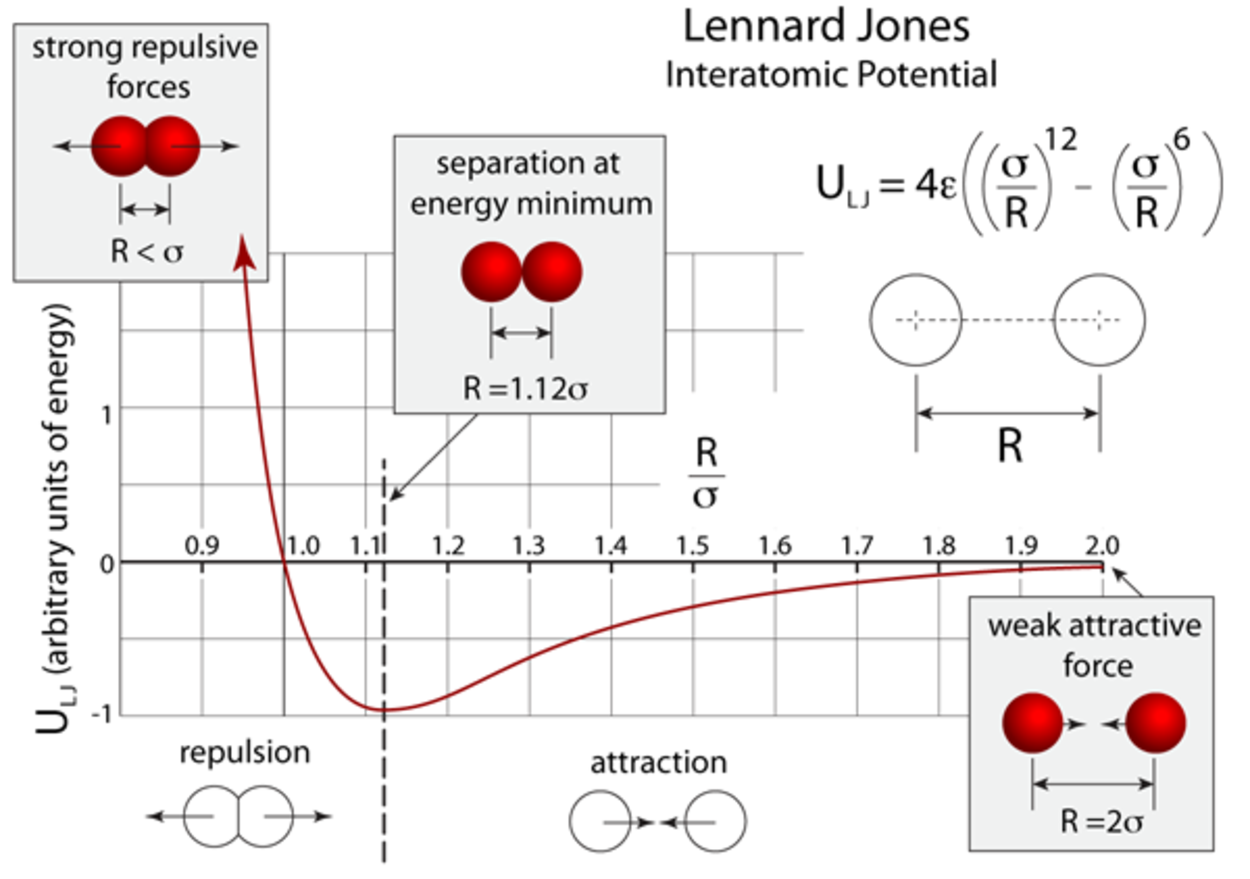
\includegraphics[width=0.8\textwidth]{pics/Lennard_Jones}
  \captionof{figure}{Lennard Jones potential \citep{atoms_in_motion}}
  \label{fig:lennard jones}
\end{figure}

Another very important form of potential typically used to describe the interaction between molecules is the \emph{Lennard Jones} potential (see fig.\ref{fig:lennard jones}). Here $\epsilon$ denotes the attractive energy and $\sigma$ is the interaction range in some arbitrary units. It is a mathematically simple model that approximates the spherical symmetric interaction between a pair of neutral atoms or molecules quite well.


\subsubsection*{Equation of motion:}
Once the interaction potential has been defined we can easily derive the equations of motion using the Hamilton equations:

$$
\dot{\vec{q}}_i^{\,k} =  \pder{\mathcal{H}}{\vec{p}_i^{\,k}},
\hspace{0.2cm}
\dot{ \vec{p}}_i^{\,k} = - \pder{\mathcal{H}}{\vec{q}_i^{\,k}},
\hspace{0.2cm} \text{with} \hspace{0.2cm}
k\in\mkl{1,...,\alpha}
\hspace{0.2cm} \text{and} \hspace{0.2cm}
i\in\mkl{1,...,N}.
$$
In the standard representation ($\vec{q}=\vec{x}$ and $\vec{p}=\vec{v}=\frac{\vec{p}}{m}$) we obtain 

\begin{equation}
\dot{\vec{p}}_i = - \nabla V\kl{Q} =f_i
\hspace{0.2cm} \text{and} \hspace{0.2cm}
m_i \ddot{\vec{x}}_i = f_i = \sum_j {f_{i,j}},
\label{newt_MD_eq}
\end{equation}

where ${f_{i,j}}$ is the force exerted by particle $j$ on particle $i$.

Those are the equations of motion to solve, which can be done by applying various numerical integration techniques (some of them already know from \citet{comp_phys}). When computing the motion of the particles, we should also estimate the precision needed and achieved by our algorithms. As an example of a numerical error, when $\Delta t$ is too large (relatively to the particles' speed), the large integration step causes numerical errors. Intuitively, for too large time steps, particles can pass through other particles' range of interaction without feeling any influence. We therefore need an estimation of the appropriate time step and of the integration error. Such a measure is the \textit{contact time}.

\subsection{Contact time:}
\label{subsec:contact_time}

Since we are only interested in a spherically symmetric interaction that solely depends on distance, we may also reduce our problem to one dimension. Using the equations for energy
$$
E= \frac{1}{2} m\dot{r}^2 + V\kl{r} = \text{constant}
$$ 
and radial velocity
$$
\der{r}{t} = \ekl{\frac{2}{m} \kl{E-V\kl{r}}}^{\frac{1}{2}},
$$
we can derive the contact time

\begin{equation}
t_c \equiv 2\int_0^{\frac{1}{2}t_c} {\text{dt}} = 
2\int_{r_{min}}^{r_{max}} {\der{t}{r}\text{dr}} =
2\int_{r_{min}}^{r_{max}} {    \ekl{\frac{2}{m} \kl{E-V\kl{r}}}^{-\frac{1}{2}}  \text{dr}}.
\label{eq:contact_time}
\end{equation}
$t_c$ can be now used to determine the appropriate time step of the simulation. The time integration of the equations of motion can be done using different schemes:
\begin{itemize}
\item Euler method
\item Runge Kutta method
\item Predictor-Corrector method
\item Verlet method
\item Leap-frog method
\end{itemize}
Here, we will only discuss the last two, which have been developed especially for Newton's equations.















